\documentclass{standalone}

\usepackage{times}
\usepackage{amsmath}
\usepackage{amssymb}

\usepackage[dvipsnames]{xcolor}
\usepackage{tikz}
\usetikzlibrary{arrows,backgrounds,scopes}

\usepackage{pgfplots}
\pgfplotsset{compat=1.15}

%ICPC logo colors
\definecolor{red}{HTML}{972e21}
\definecolor{yellow}{HTML}{ebb83f}
\definecolor{blue}{HTML}{5e7fbf}
\definecolor{green}{HTML}{5fd94e}

\begin{document}
	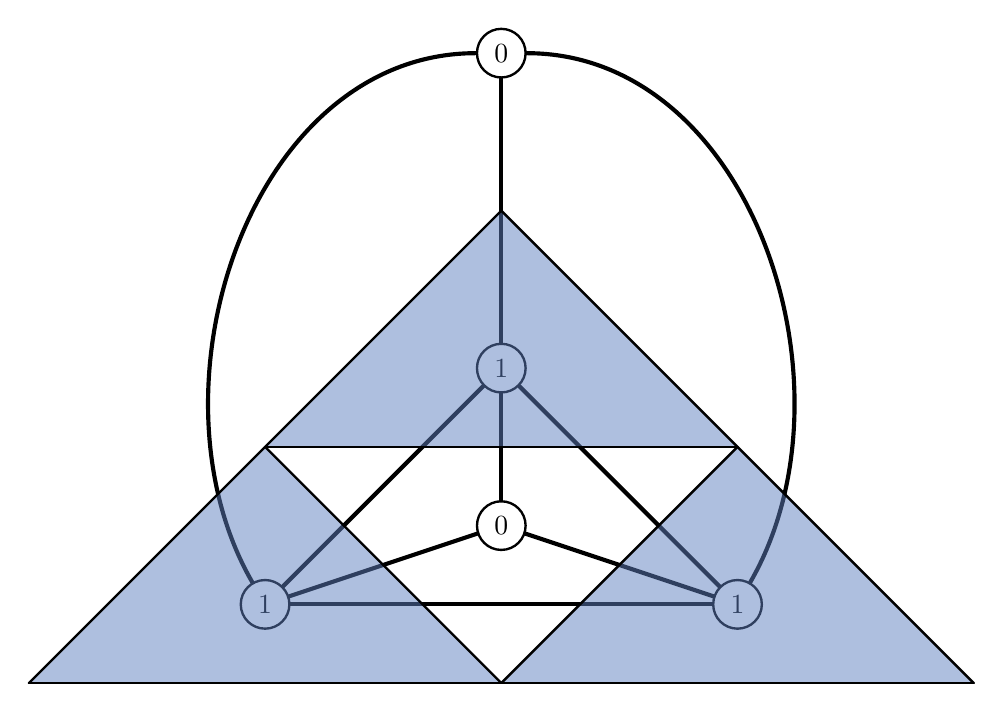
\begin{tikzpicture}[every path/.style={line cap=round, line width=0.03cm}]
		
			
        \tikzset{vertex/.style = {shape=circle,draw,minimum size=1.5em}}
        \tikzset{edge/.style = {}}

        \node[vertex] (1) at (0,1) {1};
        \node[vertex] (2) at (-3,-2) {1};
        \node[vertex] (3) at (0,-1) {0};
        \node[vertex] (4) at (3,-2) {1};
        \node[vertex] (5) at (0,5) {0};
        \draw[edge, line width=1.5pt] (1) to (2);
        \draw[edge, line width=1.5pt] (1) to (3);
        \draw[edge, line width=1.5pt] (1) to (4);
        \draw[edge, line width=1.5pt] (2) to (3);
        \draw[edge, line width=1.5pt] (2) to (4);
        \draw[edge, line width=1.5pt] (3) to (4);

        \draw[edge, line width=1.5pt] (5) to [out=180, in=120] (2);
        \draw[edge, line width=1.5pt] (5) to (1);
        \draw[edge, line width=1.5pt] (5) to [out=0, in=60] (4);


        %\draw[edge, line width=1.5pt] (15) to [out=-50, in=-130] (13);

        \fill[blue,opacity=0.5] (-3,0) -- (0,-3) -- (-6,-3) -- cycle;
        \fill[blue,opacity=0.5] (-3,-0) -- (3,0) -- (0,3) -- cycle;
        \fill[blue,opacity=0.5] (3,0) -- (6,-3) -- (0,-3) -- cycle;
        % \fill[white,opacity=0.3] (-3,0) -- (3,0) -- (0,-3) -- cycle;
			
        \draw (-6,-3) -- (0,3);
        \draw (0,3) -- (6,-3);
        \draw (6,-3) -- (-6,-3);
        \draw (-3,0) -- (3,0);
        \draw (3,0) -- (0,-3);
        \draw (0,-3) -- (-3,0);		
	\end{tikzpicture}
\end{document} 
